\documentclass[11pt]{article}

\usepackage{tikz}
\usepackage{kotex}

\usetikzlibrary{arrows.meta}

\begin{document}
Hello world? One


\begin{tikzpicture}
\tikz{\draw (0,0) rectangle (2ex, 1em)}
\tikz[very thick] \draw (0,0) rectangle (2ex, 1em); \\
\tikz \draw (0pt, 3pt) -- (20pt, 3pt);
\end{tikzpicture}

\begin{tikzpicture}
\tikz \draw (0pt, 3pt) -- (20pt, 3pt);
\end{tikzpicture}

\begin{tikzpicture}
\tikz \draw[>-] (0pt, 3pt) -- (20pt, 3pt);
\end{tikzpicture}

\begin{tikzpicture}
\tikz \draw[->] (0pt, 3pt) -- (20pt, 3pt);
\end{tikzpicture}

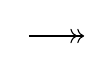
\begin{tikzpicture}
\tikz \draw[->>] (0pt, 3pt) -- (20pt, 3pt);
\end{tikzpicture}

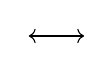
\begin{tikzpicture}
\tikz \draw[<->] (0pt, 3pt) -- (20pt, 3pt);
\end{tikzpicture}

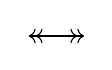
\begin{tikzpicture}
\tikz \draw[<<->>] (0pt, 3pt) -- (20pt, 3pt);
\end{tikzpicture}

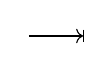
\begin{tikzpicture}
\tikz \draw[->|] (0pt, 3pt) -- (20pt, 3pt);
\end{tikzpicture}

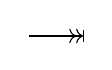
\begin{tikzpicture}
\tikz \draw[->>|] (0pt, 3pt) -- (20pt, 3pt);
\end{tikzpicture}

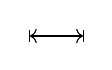
\begin{tikzpicture}
\tikz \draw[|<->|] (0pt, 3pt) -- (20pt, 3pt);
\end{tikzpicture}

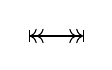
\begin{tikzpicture}
\tikz \draw[|<<->>|] (0pt, 3pt) -- (20pt, 3pt);
\end{tikzpicture}

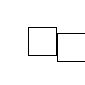
\begin{tikzpicture}
\tikz \draw (0,0) rectangle (1em, 1em);
\tikz[baseline=2pt] \draw (0, 0) rectangle (1em, 1em);
\end{tikzpicture}

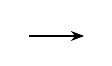
\begin{tikzpicture}
\tikz \draw[-Stealth] (0pt, 3pt) -- (20pt, 3pt);
\end{tikzpicture}

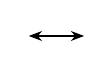
\begin{tikzpicture}
\tikz \draw[Stealth-Stealth] (0pt, 3pt) -- (20pt, 3pt);
\end{tikzpicture}

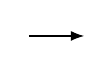
\begin{tikzpicture}
\tikz \draw[-Latex] (0pt, 3pt) -- (20pt, 3pt);
\end{tikzpicture}

\begin{tikzpicture}
\tikz \draw[-{Classical TikZ Rightarrow}] (0pt, 3pt) -- (20pt, 3pt);
\end{tikzpicture}

\tikz{\draw[-{Stealth[length=3mm]}](0,0)--(1.2,0);
\draw[|<->|](0.8,.4) -- node[above=1mm]{3mm}(1.2,.4);}

\tikz{\draw[-{Latex[length=3mm]}](0,0)--(1.5,0);
\draw[|<->|](0.8,.4) -- node[above=1mm]{3mm}(1.2,.4);}

\tikz{\draw[-{Classical TikZ Rightarrow [length=3mm]}](0,0)--(1.2,0);
\draw[|<->|](0.8,0.6) -- node[above=1mm]{3mm}(1.2,.6);}

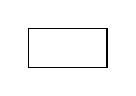
\begin{tikzpicture}
\draw rectangle (1,0.5);
\end{tikzpicture}

\begin{tikzpicture}[x=2, y=1, z=2]
\draw rectangle (2,3);
\end{tikzpicture}

\begin{tikzpicture}[x={(2mm,0)}, y={(0,1mm)}]
\draw rectangle (2,3);
\end{tikzpicture}

\tikz{\draw[line width=5pt] (0,0) -- (1cm, 1.5ex);}
\tikz{\draw[ultra thin] (0,0) -- (1cm,1.5ex);}
\tikz{\draw[very thin] (0,0) -- (1cm, 1.5ex);}
\tikz{\draw[thin] (0,0) -- (1cm,1.5ex);}
\tikz{\draw[semithick] (0,0) -- (1cm, 1.5ex);}

\tikz{\draw[thick] (0,0) -- (1cm, 1.5ex);}
\tikz{\draw[very thick] (0,0) -- (1cm, 1.5ex);}
\tikz{\draw[ultra thick] (0,0) -- (1cm, 1.5ex);}
\tikz{\draw[dash pattern=on 20pt off 3pt on 4pt off 4pt] (0pt, 0pt) -- (50pt, 8pt);}
\tikz{\draw[dash pattern=on 20pt off 8pt, dash phase=0pt](0pt, 0pt) -- (50pt, 8pt);}

\tikz{\draw[dash pattern=on 20pt off 8pt, dash phase=10pt](0pt, 0pt) -- (50pt, 8pt);}
\tikz{\draw[solid](0pt, 0pt) -- (50pt, 8pt);}
\tikz{\draw[dotted](0pt, 0pt) -- (50pt, 8pt);}
\tikz{\draw[densely dotted](0pt, 0pt) -- (50pt, 8pt);}
\tikz{\draw[loosely dotted](0pt, 0pt) -- (50pt, 8pt);}

\tikz{\draw[dashed](0pt, 0pt) -- (50pt, 8pt);}
\tikz{\draw[densely dashed](0pt, 0pt) -- (50pt, 8pt);}
\tikz{\draw[loosely dashed](0pt, 0pt) -- (50pt, 8pt);}
\tikz{\draw[dash dot](0pt, 0pt) -- (50pt, 8pt);}
\tikz{\draw[densely dash dot](0pt, 0pt) -- (50pt, 8pt);}

\tikz{\draw[loosely dash dot](0pt, 0pt)--(50pt, 8pt);}
\tikz{\draw[dash dot dot](0pt, 0pt) -- (50pt, 8pt);}
\tikz{\draw[densely dash dot dot](0pt, 0pt) -- (50pt, 8pt);}
\tikz{\draw[loosely dash dot dot](0pt, 0pt) -- (50pt, 8pt);}

\begin{tikzpicture}[x=1cm, y=1cm]
\draw[thick, ->] (0,0) -- (5,0); % x 축
\draw[very thick, ->] (2.5, -2.5) -- (2.5, 2.5); % y 축
\draw[color=red](2.5, 0) circle (1.5);
\end{tikzpicture}

\begin{tikzpicture}[scale=1.1]
\draw node[rectangle, draw] at (0,0) {노드};
\shadedraw[draw] (2,0) circle [x radius=0.8, y radius=1];
\shade[color=white] (4,0) circle [x radius=0.8, y radius=1];
\fill[pink, draw] (6,0) circle [x radius=0.8, radius=1];
%\pattern[pattern=horizontal lines light blue, draw] (8,0) ellipse [x radius=0.8, y radius=1];
\end{tikzpicture}

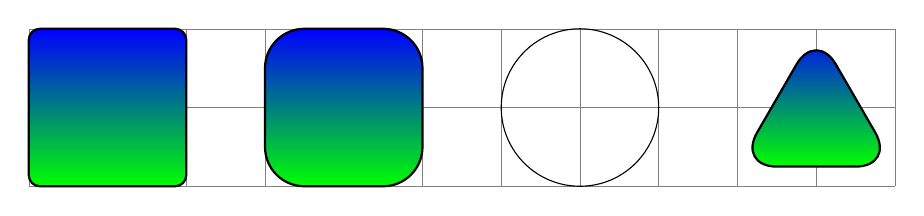
\begin{tikzpicture}
\tikzstyle mystyle=[style={thick, shade, top color=blue, bottom color=green, rounded corners=.5cm}];
\draw[help lines] (0,0) grid (11,2);
\draw[style=mystyle, rounded corners] (0,0) rectangle (2,2);
\draw[style=mystyle] (3,0) rectangle (5,2);
\draw[rounded corners=1cm](6,0) rectangle (8,2);
\draw[style=mystyle] (9, 0.25) -- (11, 0.25) -- (10, 1.98) -- cycle;
\end{tikzpicture}

\begin{tikzpicture}[scale=1.3]
\draw[step=1cm, gray!70, thin] (0,0) grid (4.2, 2.2);
\draw[thick, <->] (0, 2.2) -- (0,0) -- (4.2,0);
\draw[fill, green] (2,1) circle [radius=2pt];

\node[text=red, font=\Large\bfseries] at (2,1){기본};
\node[below=3mm] at (2,1) {아래};
\node[above=2mm] at (2,1) {위쪽};
\node[left=.5cm] at (2,1) {왼쪽};
\node[right=.5cm] at (2,1) {오른쪽};
\end{tikzpicture} \\
%%
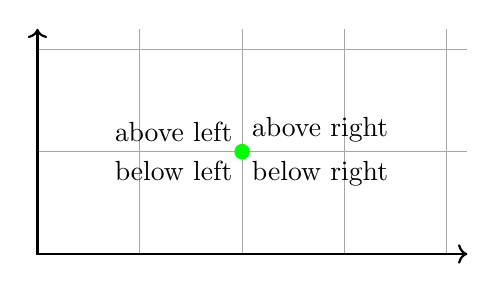
\begin{tikzpicture}[scale=1.3]
\draw[step=1cm, gray!70, thin] (0,0) grid (4.2, 2.2);
\draw[thick, <->] (0,2.2) -- (0,0) -- (4.2,0);
\draw[fill, green] (2,1) circle [radius=2pt];

\node[above left] at (2,1) {above left};
\node[above right] at (2,1) {above right};
\node[below left] at (2,1) {below left};
\node[below right] at (2,1) {below right};
\end{tikzpicture}

\begin{tikzpicture}[xscale=1.3]
\draw[step=3cm, gray!70, thin] (0, -0.2) grid (9, 0.2);
\node[align=left, below] at (1.5, -0.5){이 부분은 \\ 왼쪽으로 \\정렬되지 않을까요?};
\node[align=center, below] at (4.5, -0.5) {이 부분은\\중앙으로 \\정렬되지 않을까요?};
\node[align=right, below] at (7.5, -0.5) {이 부분은\\오른쪽으로 \\정렬되지 않을까요?};
\end{tikzpicture}

\begin{tikzpicture}
\node[fill=pink] at (0, 0) {상자};
\node[draw] at (1.5, 0) {긴 상자};
\node[draw] at (4,0) {좀 더 긴 상자};
\node[fill=pink, circle] at (6,0) {원};
\node[fill=pink, circle] at (7.5cm, 0) {중간 원};
\node[fill=pink, circle] at (9.5cm, 0) {제일 큰 원};
\end{tikzpicture}

\begin{tikzpicture}
\draw node[fill=yellow, draw, circle, text width=1.5cm] at (0,0) {원};
\draw node[fill=yellow, draw, circle, text width=1.5cm] at (2,0) {중간 원};
\draw node[fill=yellow, draw, circle, text width=1.5cm] at (4,0) {큰 원};
\draw node[fill=pink, draw=blue, circle, text width=1.5cm, align=center] at (6,0) {원};
\draw node[fill=pink, draw=blue, circle, text width=1.5cm, align=center] at (8,0) {중간 원}
\draw node[fill=pink, draw=blue, circle, text width=1.5cm, align=center] at (10,0) {큰 원}
\end{tikzpicture}


\end{document}